\documentclass[12pt, %
openright, 
oneside,
a4paper,
brazil]{facom-ufu-abntex2}
\usepackage{xcolor}
% Definindo novas cores
\definecolor{verde}{rgb}{0.25,0.5,0.35}
\definecolor{jpurple}{rgb}{0.5,0,0.35}
% Configurando layout para mostrar codigos Java
\usepackage{listings}
\usepackage{longtable}
\lstset{
  language=Java,
  basicstyle=\ttfamily\small, 
  keywordstyle=\color{jpurple}\bfseries,
  stringstyle=\color{red},
  commentstyle=\color{verde},
  morecomment=[s][\color{blue}]{/**}{*/},
  extendedchars=true, 
  showspaces=false, 
  showstringspaces=false, 
  numbers=left,
  numberstyle=\tiny,
  breaklines=true, 
  backgroundcolor=\color{cyan!10}, 
  breakautoindent=true, 
  captionpos=b,
  xleftmargin=0pt,
  tabsize=4
}
\autor{Patrick Godinho} %TCC
\data{2014}
\orientador{Lasaro Camargos} %TCC
%\coorientador{Algum?} %TCC 


\usepackage{todonotes}


% ---
% Informações de dados para CAPA e FOLHA DE ROSTO
% ---

\titulo{PheroCast App} %TCC

\hypersetup{pdfkeywords={palavra 1}{palavra 2}{palavra 4}{palavra 4}{palavra 5}} %TCC

\begin{document}
\frenchspacing 

% ----------------------------------------------------------
% ELEMENTOS PRÉ-TEXTUAIS
% ----------------------------------------------------------
%\pretextual
\imprimircapa
\imprimirfolhaderosto


% ---
% Inserir folha de aprovação
% ---
%
% \includepdf{folhadeaprovacao_final.png} %TCC: depois de aprovado o trabalho, descomente esta linha e comente o próximo bloco para incluir scan da folha de aprovação.
%
\begin{folhadeaprovacao}

  \begin{center}
    {\ABNTEXchapterfont\large\imprimirautor}

    \vspace*{\fill}\vspace*{\fill}
    {\ABNTEXchapterfont\bfseries\Large\imprimirtitulo}
    \vspace*{\fill}
    
    \hspace{.45\textwidth}
    \begin{minipage}{.5\textwidth}
        \imprimirpreambulo
    \end{minipage}%
    \vspace*{\fill}
   \end{center}
    
   Trabalho aprovado. \imprimirlocal, 24 de novembro de 2012: %TCC:

   \assinatura{\textbf{\imprimirorientador} \\ Orientador}  
   \assinatura{\textbf{Professor}}% \\ Convidado 1} %TCC:
   \assinatura{\textbf{Professor}}% \\ Convidado 2} %TCC:
   %\assinatura{\textbf{Professor} \\ Convidado 3}
   %\assinatura{\textbf{Professor} \\ Convidado 4}
      
   \begin{center}
    \vspace*{0.5cm}
    {\large\imprimirlocal}
    \par
    {\large\imprimirdata}
    \vspace*{1cm}
  \end{center}
  
\end{folhadeaprovacao}
% ---


%%As seções dedicatória, agradecimento e epígrafe não são obrigatórias.
%%Só as mantenha se achar pertinente.

% ---
% Dedicatória
% ---
\begin{dedicatoria}
   \vspace*{\fill}
   \centering
   \noindent
   \textit{Dedico a meu pai Paulo Sergio de Jesus Oliveira que sempre foi um exemplo de perseverança na minha vida!}  %TCC:
   \vspace*{\fill}
\end{dedicatoria}
% ---

% ---
% Agradecimentos
% ---
\begin{agradecimentos}
Agradeço a Deus, minha esposa e ao meu orientador Lasaro Camargos pelo apoio e dedicação para que eu conseguisse chegar ao final deste trabalho. %TCC:
\end{agradecimentos}
% ---

% ---
% Epígrafe
% ---
%\begin{epigrafe}
%    \vspace*{\fill}
%	\begin{flushright}
%		\textit{``Alguma citação que ache conveniente? \lipsum[10]''} %TCC:
%	\end{flushright}
%\end{epigrafe}
% ---



\begin{resumo} %TCC:
Com o objetivo de melhorarmos os algoritmos de predição da localização de um nó em uma ambiente de redes móveis, necessitamos de dados reais como os que foram gerados através do produto final desse trabalho, o PheroCast App. Um aplicativo Android que coleta as redes sem fio ao alcance do dispositvo e armazena para futuras análises.
 \todo[inline]{Informal demais. Siga a mestra estrutura do documento: contexto, justificativa, resultados.}
 \vspace{\onelineskip}
    
 \noindent
 \textbf{Palavras-chave}: Manet, Vanet, Android, Predição de Localização%TCC:
\end{resumo}

% ---
% inserir lista de ilustrações
% ---
\pdfbookmark[0]{\listfigurename}{lof}
\listoffigures*
\cleardoublepage
% ---

% ---
% inserir lista de tabelas
% ---
\pdfbookmark[0]{\listtablename}{lot}
\listoftables*
\cleardoublepage
% ---



% ---
% inserir lista de abreviaturas e siglas
% ---
%\begin{siglas} %TCC:
%  \item[Fig.] Area of the $i^{th}$ component
%  \item[456] Isto é um número
%  \item[123] Isto é outro número
%  \item[Zézão] este é o meu nome
%\end{siglas}
% ---

%% ---
%% inserir lista de símbolos, se for adequado ao trabalho. %TCC:
%% ---
%\begin{simbolos}
%  \item[$ \Gamma $] Letra grega Gama
%  \item[$ \Lambda $] Lambda
%  \item[$ \zeta $] Letra grega minúscula zeta
%  \item[$ \in $] Pertence
%\end{simbolos}
%% ---

% ---
% inserir o sumario
% ---
\pdfbookmark[0]{\contentsname}{toc}
\tableofcontents*
\cleardoublepage
% ---





% ----------------------------------------------------------
% ELEMENTOS TEXTUAIS
% ----------------------------------------------------------
\textual


% ----------------------------------------------------------
% Introdução
% ----------------------------------------------------------

\chapter{Introdução}
\addcontentsline{toc}{chapter}{Introdução}
%TCC:
\section{Contextualização}
\subsection{MANET}
MANET é a abreviação de Mobile Ad-Hoc Networks, a qual se define pelas redes em que nós se movimentam livremente, comunicam entre si e entre o meio em que está, sem a necessidade de nenhuma infraestrutura de rede. Tais ações permitem que várias aplicações sejam desenvolvidas com objetivo por exemplo da troca de informações entre os nós ou até o compartilhamento de serviços, como por exemplo a funcionalidade que temos hoje em dia de rotear a internet do celular com dispositivos próximos.


Tambem definida por MANET pode ser conceituada como um sistema autonomo de servidores moveis (que tambem servem de roteadores), os quais unidos formam uma rede de comunicacao representada por um grafo.
\todo[inline]{Diversos erros de acentuacao, concordancia e, o pior, a frase nao faz muito sentido.}

Os nós em uma MANET se movem arbitrariamente, e essa é a grande característica da rede, mas também o principal ofensor na qualidade da comunicação disponibilizada nesse ambiente, pois a arquitetura entre eles deve sempre estar se adaptando para os novos meios em que estão inseridos.
\cite{de2002mobile}

Desde que surgiu, a MANET tem sido vista como uma das mais desafiantes abordagens de redes móveis tanto pela promessa de crescimento de dispositivos móveis, quanto pela sua complexidade, o que impulsionou a pesquisa por esse paradigma. Apartir das pesqusias intensas na MANET, surgiram outras redes móveis baseadas em sua proposta inicial. Como por exemplo a VANET que será introduzida na próxima seção.



\subsection{VANET}
\subsubsection{Conceito}
VANET são redes móveis MANET onde os nós são os veículos e até a estrada, onde há comunicação apenas entre os automóveis (IVC - Inter Vehicle Communication), ou entre os mesmos e a estrada (RVC - Road Vehicle Communication).

Assim como na MANET, a Vehicular Ad-Hoc Network também permite que várias aplicações com vários objetivos sejam desenvolvidos, bem como alertar obstáculos na estrada, broadcast de informações de segurança, compartilhar informações de tráfego ou até solicitar socorro em algum acidente.

As simualções e experimentos tem tido um papel importante no desenvolvimento das soluções para redes veiculares. A atenção maior tem sido dada no desenvolvimento de modelos realistas de estrada e principalmente no estudo da mobilidade dos veículos. Por exemplo, modelos de como os carros se movem ao longo do trajeto, levando em consideração sua velocidade, sinais de transito, dentre outros fatores. 

\subsubsection{Problema}
O grande desafio das Redes Ad-Hoc Veiculares é o roteamento entre os nos, devida a alta taxa de mobilidade dos veículos que são conectados entre si intermitentemente, dificultando a entrega das mensagens entre os  ou estrada, pois frequentemente um nó muda seu endereço, ficando assim diferente de qual se identificou.

Alem do problema citado acima, existe um agravante relacionado a velocidade de conexão entre os , os quais se comunicam muito rápido, levando em consideração que os mesmos estejam em uma via rápida.

\subsection{Predição de localização}
\subsubsection{Motivo}
A predição da localidade de um nó, o qual pode ser um automóvel, uma pessoa com um dispositivo móvel, é algo bastante motivador a se desenvolver pelo fato de trazer otimizações da comunicação das redes MANET e suas derivadas, através da gestão proativa. \cite{6838650}
\todo[inline]{Portugues horrível. }

Por exemplo, caso um nó mande uma requisição para outro e logo após mude de localização, o responsável pela resposta será proativo o bastante para saber em qual posição o destinatário estará, resolvendo assim o problema da mobilidade, o qual é o principal desafio da VANET.
\todo[inline]{Isso não é automático dado a predição. Predição só possibilita, mas ainda precisa ser desenvolvido.}

A predição de localização também é alvo de escopo de várias aplicações com o objetivo por exemplo de prever e otimizar tráfego em cidades inteligentes, ou até prever potenciais clientes para um passeio ecológico.

\subsubsection{PheroCast}
\paragraph{Conceito}
PheroCast é o nome que se deu à abordagem de previsão da localização futura de um nó em uma rede ad-hoc móvel. Foi nomeado assim pela semelhança com o fenomeno que acontece na colonia das formigas, o qual para alertar problemas, ou marcar o caminho, por onde a formiga passar, ela deixará um rastro, formando assim um caminho.

Nessa abordagem, o algoritmo de previsão é desenvolvido para ser processado nos próprios nós móveis. Assim, a cada intervalo de tempo definido, o nó registra um rastro de onde está. Daí vem a semelhança com o ``Pheronomium'' \todo{forma correta de se colocar aspas em latex.} deixado no rastro por onde a formiga passa.

Assim, com o histórico dos "traces" de um determinado nó na forma de um grafo, é possível determinar uma probabilidade de onde ele estará em determinado horário apartir de um certo lugar.

\paragraph{Resultados}
Segundo \cite{6838650} foi feita uma avaliação do algoritmo PheroCast usando os caminhos dos onibus de Seattle Metro Transit, que vale a pena ressaltar, não foram extraídos para a abordagem nem com o intervalo de tempo ideal. Foi descoberto que a abordagem obteve bons resultados em relação à predição das futuras posicões dos onibus. A avaliação obteve 77,8\% de resultados positivos. \todo[inline]{Este trabalho já foi extendido no mestrado o enrique fynn. entre em contato e pegue as atualizações com ele.}

\paragraph{Problema}
O grande problema do PheroCast é a sua avaliação limitada, ou seja, é necessário, para uma abordagem com essas características, uma avaliação extensa com dados reais, que ssimulam de verdade a mobilidade humana. 

Atualmente não existem "traces" reais, e sim módulos de mobilidade sintéticos, os quais não são realistas. Daí vem a proposta deste trabalho, o qual irá cooperar para avaliação confiável do PheroCast, coletando dados de mobilidade humana reais, através de seus dispositivos móveis.
\section{Proposta}
A proposta deste trabalho é desenvolver um sistema que rode em dispositivos móveis, para capturar "traces" reais de mobilidade humana. Para tal, o sistema irá coletar em um intervalo de tempo, todas as redes wireless, bem como suas informações, ao redor do dispositivo móvel do usuário e armazenar em um servidor para que os dados sejam compilados e utilizados para avaliação do PheroCast.

O objetivo é que o sistema seja utilizado por mais de um usuário para que assim tenhamos grande diversidade de histórico de traces.

\todo{mal escrito.}

\chapter{Referencial Teórico}
\section{PheroCast}

	O PheroCast, conjunto de algoritmos para prever a localização de um nó em alguma rede móvel, foi desenvolvido por um grupo de pesquisa da Universidade Federal de Uberlândia, o The Distributed Systems and Networks  Research Group, criado em 2013, constituído de doutores, mestres e alunos da Faculdade de Computação. citar grupo. 
	
	Nosso objetivo nessa seção não é de descrever o algoritmo bem como seus passos, cálculos e funções, e sim, explicar o conceito do algoritmo e seus principais componentes. Tais assuntos foram utilizados para o desenvolvimento deste trabalho.
	
	Para entedermos a abordagem do Pherocast, que consiste na previsão da posição dos nós de uma rede móvel baseada no conceitos dos feromônios, vamos conceituar e exemplificar alguns componentes utilizados pelo algoritmo.

	Como as formigas passam a vida em contato com o solo, em suas caminhadas, elas deixam um rastro de feromônio que pode ser seguida por ouras formigas. Trazendo para o nosso contexto, um nó em uma rede móvel pode sinalizar os pontos em que passou, e assim construir um caminho que percorreu de um ponto a outro. Podemos também afirmar com esse conceito que um nó está em uma localização X se X é o sinal mais perto de sua posição.
	
	\cite{6838650} Cada marca, ou log deixado pelo nó contém a informação da localização e a hora em que passou por ele, e a direção  tornando assim análises como a velocidade do nó, ou a grandeza da localização. Por exemplo, caso um nó sinalize que está em uma localização em vários intervalos de tempo consecutivos, podemos concluir que essa localização, ou área de alcance é grande, ou que o nó está em baixa velocidade. Por outro lado, caso uma localização é pouco marcada, o nó pode estar em uma alta velocidade ou a área é pequena, onde pouco "feromônio" foi liberado.
	
	No PheroCast esses sinais que contém a localização e a hora, são convertidos em Phero Trails, um dígrafo que contém como vértices os locais visitados pelos nós, e a direção em que estão (norte, sul, leste, oeste) ligados  por arestas de forma em que represente a movimentação do nó, e assim seu caminho o qual possui uma localização inicial e uma final.
	
	Com os Phero Trails definidos, temos a capacidade de utilizar um dos algoritmos do PheroCast e traçar o que chamamos de Phero Maps, dígrafos que contém além da localização e a direção, a quantidade de vezes que o nó passou por ali, ligados por arestas que indicam a próxima localização que o nó passou, e assim por diante. Assim conseguimos concluir que para chegar em uma localização final, o nó passou por diversos caminhos diferentes, também definimos as possíveis rotas entre um determinado ponto e outro.
	
	Dado um Phero Map definido, temos todas as variáveis que o algoritmo de previsão de uma futura localização do nó, descrita no Phero Cast necessita. Tais elas são: localização, direção, quantidade de vezes que passou pela localização. 
	
 	O produto final desse trabalho, tem como objetivo produzir dados reais de localização, tratando os feromônios como registros de rede wifi,registrados pelo dispositivo móvel em um determinado intervalo de tempo, e armazenando em um local para ser reproduzidas em mapas e diagramas, como aborda o Phero Cast.
	

\section{Android}

	Para o desenvolvimento desse trabalho, utilizamos o sistema operacional Android, baseado em Linux que opera em celulares, netbooks, tablets, dentre outros dispositivos. O Android nos fornece um robusto framework de aplicação que nos permite implementar aplicações para dispositivos móveis utilizando Java.
	

	Tal framework disponibiliza alguns componentes, os quais alguns deles foram utilizados na construção desse trabalho.
	Iremos detalhar cada componente a seguir:
	\cite{googleand}
	
	\subsection{Activities}
	O componente Activity representa uma única tela com interface para o usuário. Por exemplo, imaginemos um aplicativo de lista de compras, iremos ter uma Activity para exibir a lista de compras, outra activity para adicionar um novo produto na lista de compras, e outra para exibir um relatório de quanto gastamos no mês.
	Uma Activity é implementada no código do aplicativo extendendo a classe Activity do Android.
	
	\subsection{Services}
	Service é o componente que roda em background no Android, podendo processar longas operações ou processar algum processo remoto. Um service não é responsável por fornecer interface para o usuário. Para entendermos melhor o funcionamento do Service, podemos exemplificar com o processo de tocar música enquanto se navega em outro aplicativo.
	Um Service é implementado no código do aplicativo extendendo a classe Service do Android.
	
	\subsection{Content Providers}
	Os Content Providers são parte importantíssima da arquitetura de um sistema android. É responsabilidade deles prover às aplicações o conteúdo que elas precisam para funcionar, ou seja, os dados.

As aplicações poderiam muito bem acessar diretamente um banco de dados, por exemplo. Porém, é uma boa prática tornar o modo como os dados são gravados transparente à aplicação. 

Além disso, essa técnica permite a criação de Shared Content Providers, que são providers “públicos” que podem ser acessados por várias aplicações. Por exemplo, existe o content provider de SMS/MMS que permite a qualquer aplicação ler as mensagens recebidas por um telefone celular.

	\subsection{Broadcast receivers}
	O Broadcast Receiver é o componente responsável por receber as mensagens broadcast do Sistema Operacional, por exemplo anúncios de que a tela foi desligada, ou a bateria está com pouca carga, ou uma foto foi tirada, ou algo na rede foi alterado. Esse componente, não fornece telas para o usuário, mas é possível criar uma barra de notificação através dele.

	\subsection{Arquivo Manifest}
	Para que o Android consiga iniciar um componente da aplicação, o sistema deve saber que esse componente existe através do arquivo AndroidManifest.xml. A aplicação desenvolvida deve conter as declarações de todos os componentes nesse arquivo, o qual está sempre localizado na pasta raíz do projeto.		


\todo{falar sobre redes sem fio wifi.}

\chapter{Proposta}
\todo{esta secao toda esta muito mal escrita para a versao final.}

\section{Arquitetura}
A arquitetura proposta consiste em duas partes, clente e servidor. O cliente é responsável pela coleta dos dados, como posição atual, lista de SSID visíveis, e quaisquer outros dados que se deseje capturar. Oportunisticamente o cliente enviará os dados ao servidor. O servidor deverá consumir os dados enviados pelo dispositivo através de uma interface REST implementada e armazenar em um banco de dados, como mostra na Figura 1.  A seguir detalhamos cada um das partes.

\begin{figure}[hbt]
  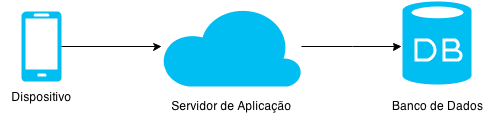
\includegraphics{arquiteturaProposta}
  \caption{Arquitetura Proposta}
\end{figure}


\subsection{Cliente}
Do lado do cliente desenvolveremos \todo{voce esta escrevendo a versao final, nao o projeto.}um sistema para rodar em dispositivos com o sistema operacional Android, utilizando a linguagem Java.

\begin{figure}[hbt]
  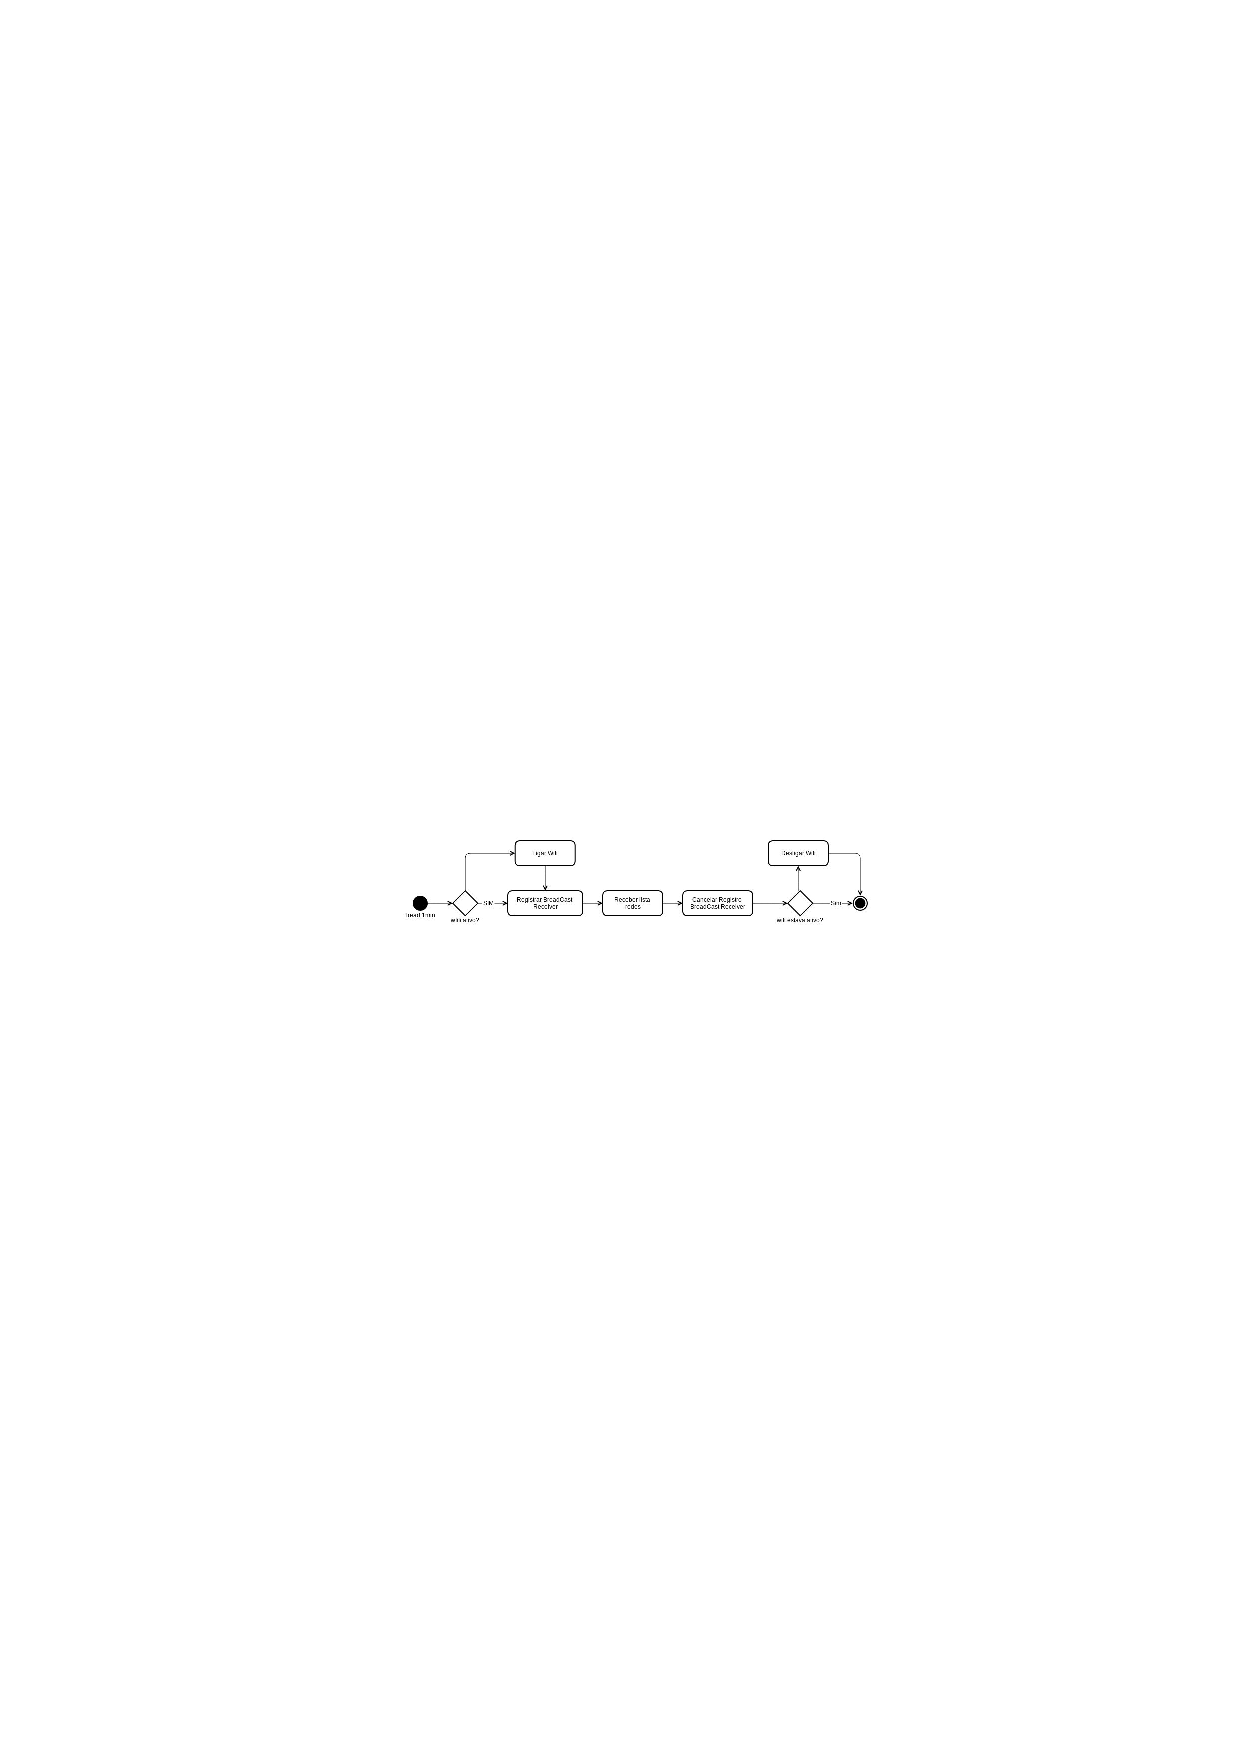
\includegraphics [scale=.4] {pherocast1}
  \caption{Processo de captura dos dados pelo aplicativo.}
\end{figure}

O aplicativo irá utilizar os serviços de Wifi do aparelho para realizar a coleta dos pontos de rede que estão ao redor naquele determinado momento. Após coleta, o sistema irá armazenar em base de dados local do dispositivo, para isso utilizaremos o banco de dados SQLite. Tal procedimento é ilustrado na Figura 2.

Para realizar o envio ao servidor, o aplicativo será alertado quando o dispositivo se conectar a uma rede WiFi com rede Internet, assim irá enviar os dados armazenados em sua base local para o servidor de aplicação na nuvem e apagar os mesmos. 

Caso o serviço de WiFi esteja desligado, o aplicativo deverá ser responsável por após ligar o Wifi e coletar os dados, desligar o mesmo, voltando assim para o estado inicial antes da coleta. Fazendo com que assim, não haja alteração no funcionamento do aparelho.




\subsection{Servidor}
Para o servidor, propomos utilizar algum servidor na nuvem de alta escalabilidade e alta disponibilidade, por se tratar de inserções contínuas todo o tempo.

O servidor deverá armazenar as informações virão do cliente, como:
\begin{itemize}
  \item SSID
  \item BSSID
  \item Recursos
  \item Frequencia
  \item Level
  \item Horário
  \item Identificador do Usuário do Dispositivo
  \end{itemize}
  
\subsection{Limpeza dos dados}
O sistema deverá tratar os dados do cliente com anonimidade, ou seja deverá haver algoritmos de segurança que tornem os dados do cliente anonimos, para preservar a identidade do usuário.


\chapter{Desenvolvimento}

\todo{Descreva o trabalho em mais detalhes. detalhes de implementacao.}
\section{Aplicativo}
Como já mencionado, o produto final deste trabalho foi um aplicativo para dispositivos Android, o qual armazena periodicamente as redes wireless disponíveis em seu alcance, e disponibiliza em um certo momento essas informações na nuvem.

Para tal, utilizamos a API do Android para operações que envolveu o funcionamento do dispositivo, como por exemplo, a coleta das redes em alcance, o sinal de que foi encontrado uma rede com internet, a ação de desligar e ligar o receptor wifi do aparelho, dentre outras operações. Além disso, implementamos o código orientado a objetos, onde cada rede coletada foi representada por um objeto.

Foram utilizadas também classes que auxiliam nas funcionalidades do aplicativo, como por exemplo, o armazenamento em uma base de dados do dispositivo, o envio dos dados para a nuvem, a identificação do usuário pelo e-mail cadastrado no dispositivo.

Abaixo detalharemos cada classe do código, com o objetivo de entendermos a estrutura do desenvolvimento do aplicativo.

Começaremos pela MainActivity, classe estendida do componente Activity do Android, o qual foi detalhado no nosso referencial teórico, que é a nossa principal classe, ou seja código responsável pela inicialização e processamento do aplicativo, através do método onCreate(). Esse método cria uma tarefa agendada que roda em intervalos de um minuto. Tal tarefa, é responsável por verificar a situação do Wifi do aparelho, e, caso este esteja desligado, é ligado. Toda essa verificação do Wifi, é feita no método getWifiState().

  Após tratar a situação do sinal wireless do aparelho, a tarefa registra através de um Intent, a classe WifiScanReceiver estendida do componente BroadCastReceiver, responsável por receber o resultado da varredura das redes wireless ao alcance do aparelho realizada.
 
 A responsabilidade da coleta das redes sem fio é do objeto instanciado da classe WifiManager da API do Android, o qual é executado através do método startScan(), após a tarefa registrar o receptor das redes encontradas.
 
  Ao receber a lista de redes através do método getScanResults da classe WifiManager, a classe WifiScanReceiver converte a lista recebida em um array de objetos da classe NetworkPoint, classe criada para representar a rede e seus atributos que são BSSID, SSID, Capabilities, Frequency, level e o momento em que foi capturada. O array de NetworkPoint é salvo na base de dados, utilizando a classe NetworkPointDAO, criada em conjunto com a PersistenceHelper, para auxiliar nas operações com o banco de dados do aplicativo, o qual foi utilizado SQLite.
 
 Importante lembrar que após o serviço de receber e armazenar as redes capturadas, a situação anterior ao processamento do sinal wireless do aparelho é mantida, ou seja, caso o aparelho esteja com a funcionalidade wifi desligada, após o processamento (que liga a mesma), a tarefa principal é responsável por desligá-la. 
 
  Para armazenar na nuvem as redes coletadas, foi utilizada a classe NetworkChangeReceiver, estendida do componente BroadCastReceiver, que tem como objetivo principal enviar um POST para o serviço de armazenamento que utilizamos através da classe HttpRequest, caso o dispositivo conecte em alguma nova rede sem fio e que a mesma tenha acesso a internet. Para cada rede armazenada no dispositivo, uma requisição POST é realizada com a informação contendo o e-mail do usuário dono do dispositivo. Tal informação é adquirida através da classe UserEmailFetcher.  Após o envio das informações da rede, a mesma é excluída da base de dados do aplicativo no dispositivo.
  

 \section{Google Docs}
Com o objetivo de simular o serviço de armazenamento na nuvem, utilizamos o Google Docs, o qual nos fornece um serviço de criação, edição e utilização de formulários de pesquisa, onde as respostas são convertidas em planilhas compartilhadas. Assim, na nossa requisição POST, com a mesma URL e parâmetros que o botão de responder o formulário que criamos com as informações esperadas das redes. Com isso, obtivemos várias linhas em planilha contendo informações das redes sem fio, a hora em que foram capturadas e o usuário responsável pela coleta.

\todo{descreva em detalhes}

\section{Limpeza dos dados}
Como tópico de trabalhos futuros, pretendemos utilizar um codificador do dado que carrega as informações do usuário, tornando assim os dados limpos e possíveis de serem colaborados com a comunidade em trabalhos que necessitem de dados reais, como no caso do PheroCast.


\chapter{Resultados}
\section{Dados Coletados}
Após divulgação do trabalho para amigos e comunidade, obtivemos mais de 45 mil registros de redes coletadas em um período de aproximadamente um mês. Compilamos os dados com apenas 5 usuários, os quais foram mais colaborativos em questão de quantidade e consideramos o suficiente para analisar os dados.
Com os dados coletados e separados por colaborador compilados em uma planilha, conseguimos o suficiente para realizar algumas análises sobre as informações adquiridas.

 Tais análises, serão exibidas na próxima seção.

\section{Análise}
Por se tratar de uma quantidade grande de dados coletados, poderíamos ter realizado diversas análises com propósitos diferentes, mas escolhemos algumas que mais relacionam com o propósito deste trabalho. Por exemplo, na Análise 1, consideramos que a rede "ALGARTELECOMVISITANTES"  seja a do local de trabalho, e a rede "Lar Doce Lar" seja a de sua residência, tmeos um cenário onde o usuário se locomoveu no dia  de um local para outro no dia 30/07/2014, coletando e armazenando as redes sem fio ao seu alcance.


 Provavelmente, o usuário do dispositivo utiliza de um caminho afastado da zona residencial, onde poucas redes foram capturadas, ou a velocidade que estava percorrendo o caminho era alta.
 
 Já na Análise 2, com redes coletadas no dia 30/07, consideramos que a rede capturada em seu local de trabalho seja a UFU-Portal e em sua residencia a "nao e sua", e tivemos um percurso com mais redes coletadas em um intervalo de tempo semelhante com a análise apresentada na Análise 1. Podemos afirmar então que o usuário da Análise 2 percorreu por um caminho com mais redes sem fio, ou que estava em baixa velocidade permitindo maior frequência de varredura das redes ao redor.


Para considerarmos que um local é o trabalho do usuário e outro é a residência, analisamos a repetição da rede coletada em um determinado intervalo de horário, por exemplo, se no horário comercial um conjunto de redes X é frequentemente capturado, pode-se afirmar que essa localização provavelmente é onde o dono do dispositivo trabalha.

% Please add the following required packages to your document preamble:
% \usepackage{graphicx}
\small
\setlength\tabcolsep{2pt}
\begin{table}
\caption{Análise 1}
\label{Análise 1}
\begin{longtable}{|c|c|c|c|c|c|}
\hline
\textbf{SSID} & \textbf{BSSID} & \textbf{Capturada em}  & \textbf{ID} \\
\hline
\endfirsthead
\multicolumn{6}{c}%
{\tablename\ \thetable\ -- \textit{Continuação da página anterior}} \\
\hline
\textbf{SSID} & \textbf{BSSID} & \textbf{Capturada em}  & \textbf{ID} \\
\hline
\endhead
\hline \multicolumn{6}{r}{\textit{Continua na próxima página}} \\
\endfoot
\hline
\endlastfoot
ALGARTELECOM\_VISITANTES  & 00:1f:ca:5f:12:73 & 30/07/2014 06:04:41 & godinhopatrick@gmail.com \\
Invicta                   & 28:10:7b:3c:31:84 & 30/07/2014 06:04:41 & godinhopatrick@gmail.com \\
Maurilio                  & 10:fe:ed:c8:ab:e6 & 30/07/2014 06:04:41 & godinhopatrick@gmail.com \\
Tudo vidros               & c8:d7:19:eb:f6:c7 & 30/07/2014 06:04:41 & godinhopatrick@gmail.com \\
b0c76a                    & 54:be:f7:70:75:4b & 30/07/2014 06:04:41 & godinhopatrick@gmail.com \\
PREMIUMHFC                & bc:f6:85:41:b3:b0 & 30/07/2014 06:04:41 & godinhopatrick@gmail.com \\
CTBC                      & 9c:d6:43:7a:fd:e3 & 30/07/2014 06:04:41 & godinhopatrick@gmail.com \\
Tudo vidros               & c8:d7:19:eb:f6:c7 & 30/07/2014 06:04:41 & godinhopatrick@gmail.com \\
HP-Print-4C-LaserJet 1102 & f4:b7:e2:3c:67:4c & 30/07/2014 06:04:41 & godinhopatrick@gmail.com \\
Tudo vidros               & c8:d7:19:eb:f6:c7 & 30/07/2014 06:04:41 & godinhopatrick@gmail.com \\
CTBC                      & 9c:d6:43:7a:fd:e3 & 30/07/2014 06:04:41 & godinhopatrick@gmail.com \\
Invicta                   & 28:10:7b:3c:31:84 & 30/07/2014 06:04:41 & godinhopatrick@gmail.com \\
ALGARTELECOM\_VISITANTES  & 00:1f:ca:5f:12:73 & 30/07/2014 06:04:41 & godinhopatrick@gmail.com \\
SPEED\_STM2               & 00:0c:42:26:73:39 & 30/07/2014 06:16:03 & godinhopatrick@gmail.com \\
SPEED\_STM2               & 00:0c:42:26:73:39 & 30/07/2014 06:16:03 & godinhopatrick@gmail.com \\
HM2 - FONE: 3084-9493     & 00:80:48:73:fb:db & 30/07/2014 06:23:01 & godinhopatrick@gmail.com \\
HM2 - FONE: 3084-9493     & 00:80:48:73:fb:db & 30/07/2014 06:23:01 & godinhopatrick@gmail.com \\
CTBC                      & 9c:d6:43:7a:bc:0b & 30/07/2014 06:25:45 & godinhopatrick@gmail.com \\
Amanda                    & c0:a0:bb:0f:68:de & 30/07/2014 06:25:45 & godinhopatrick@gmail.com \\
CTBC                      & 9c:d6:43:7a:bc:0b & 30/07/2014 06:25:45 & godinhopatrick@gmail.com \\
Amanda                    & c0:a0:bb:0f:68:de & 30/07/2014 06:25:45 & godinhopatrick@gmail.com \\
Lar Doce Lar              & c0:a0:bb:0e:fa:1e & 30/07/2014 06:28:28 & godinhopatrick@gmail.com
\end{longtable}
\end{table}

\small
\setlength\tabcolsep{2pt}
\begin{table}
\caption{Análise 2}
\label{Análise 2}
\begin{longtable}{|c|c|c|c|c|c|}
\hline
\textbf{SSID} & \textbf{BSSID} & \textbf{Capturada em}  & \textbf{ID} \\
\hline
\endfirsthead
\multicolumn{6}{c}%
{\tablename\ \thetable\ -- \textit{Continuação da página anterior}} \\
\hline
\textbf{SSID} & \textbf{BSSID} & \textbf{Capturada em}  & \textbf{ID} \\
\hline
\endhead
\hline \multicolumn{6}{r}{\textit{Continua na próxima página}} \\
\endfoot
\hline
\endlastfoot
UFU-Portal & d8:c7:c8:d5:79:41 & 04/08/2014 05:36:47 & lasaro@gmail.com \\
UFU-Portal & d8:c7:c8:d5:79:41 & 04/08/2014 05:36:47 & lasaro@gmail.com \\
DaComp & f8:1a:67:13:79:90 & 04/08/2014 05:36:47 & lasaro@gmail.com \\
dlink & 00:21:91:6f:18:00 & 04/08/2014 05:36:47 & lasaro@gmail.com \\
UFU-Portal & d8:c7:c8:d5:78:a1 & 04/08/2014 05:36:47 & lasaro@gmail.com \\
UFU-Portal & d8:c7:c8:d5:78:a1 & 04/08/2014 05:36:47 & lasaro@gmail.com \\
OpenWrt & 90:f6:52:3e:ca:58 & 04/08/2014 05:36:47 & lasaro@gmail.com \\
OpenWrt & 90:f6:52:3e:ca:58 & 04/08/2014 05:36:47 & lasaro@gmail.com \\
BENARENGE & 00:1d:1a:0a:91:ea & 04/08/2014 05:45:07 & lasaro@gmail.com \\
MM GAMA & 20:aa:4b:a9:b7:57 & 04/08/2014 05:45:07 & lasaro@gmail.com \\
b7b380 & 54:be:f7:87:b0:a7 & 04/08/2014 05:45:07 & lasaro@gmail.com \\
ultrabl\_1149\_20m & 20:aa:4b:4f:a9:ca & 04/08/2014 05:45:07 & lasaro@gmail.com \\
b13c34 & 54:be:f7:71:bc:bd & 04/08/2014 05:45:07 & lasaro@gmail.com \\
22ks & 90:f6:52:68:7c:c2 & 04/08/2014 05:45:07 & lasaro@gmail.com \\
VERTICAL\_FILMES & 20:aa:4b:d0:62:c3 & 04/08/2014 05:45:07 & lasaro@gmail.com \\
WJS & 2a:a4:3c:7d:48:52 & 04/08/2014 05:45:07 & lasaro@gmail.com \\
CLIENTE-DGUSTO & 90:f6:52:a6:36:32 & 04/08/2014 05:45:07 & lasaro@gmail.com \\
Serafim & d8:5d:4c:d6:40:2c & 04/08/2014 05:45:07 & lasaro@gmail.com \\
b0ed44 & 54:be:f7:6c:51:7b & 04/08/2014 05:45:07 & lasaro@gmail.com \\
enio & c8:be:19:01:b8:a8 & 04/08/2014 05:45:07 & lasaro@gmail.com \\
NetVirtua\_582 & 90:0d:cb:f4:97:00 & 04/08/2014 05:45:07 & lasaro@gmail.com \\
c7917c & 70:54:d2:c7:03:04 & 04/08/2014 05:45:07 & lasaro@gmail.com \\
abacaxi & 70:54:d2:c3:4c:43 & 04/08/2014 05:45:07 & lasaro@gmail.com \\
Marcio D-Link & 28:10:7b:3e:23:fb & 04/08/2014 05:45:07 & lasaro@gmail.com \\
c7184a & 70:54:d2:c6:16:bf & 04/08/2014 05:45:07 & lasaro@gmail.com \\
CAETES02 & 98:fc:11:ce:e6:ae & 04/08/2014 05:45:07 & lasaro@gmail.com \\
Viveiro Rosalia & 9c:d6:43:7b:51:d3 & 04/08/2014 05:49:33 & lasaro@gmail.com \\
EDC & 20:aa:4b:d8:84:f3 & 04/08/2014 05:49:33 & lasaro@gmail.com \\
Bom jesus & 1c:7e:e5:99:68:10 & 04/08/2014 05:49:33 & lasaro@gmail.com \\
fransergio de camargo & 84:c9:b2:cc:ce:3d & 04/08/2014 05:49:33 & lasaro@gmail.com \\
c6eb7a & 70:54:d2:c4:25:27 & 04/08/2014 05:49:33 & lasaro@gmail.com \\
versii\_ap2 & 94:0c:6d:aa:1e:e6 & 04/08/2014 05:49:33 & lasaro@gmail.com \\
HarryPotter & 64:66:b3:da:c7:95 & 04/08/2014 05:49:33 & lasaro@gmail.com \\
Advocacia & 00:1d:0f:d5:e2:de & 04/08/2014 05:49:33 & lasaro@gmail.com \\
Nasa Hi-Fi & b0:48:7a:f2:2a:5a & 04/08/2014 05:49:33 & lasaro@gmail.com \\
HP-Print-96-LaserJet 1102 & 1c:3e:84:f5:ef:96 & 04/08/2014 05:49:33 & lasaro@gmail.com \\
vargas & 20:aa:4b:d0:63:32 & 04/08/2014 05:49:33 & lasaro@gmail.com \\
Francine & c8:d7:19:60:95:90 & 04/08/2014 05:49:33 & lasaro@gmail.com \\
ALINEMAMEDE-PC\_Network & 54:e6:fc:a4:d8:48 & 04/08/2014 05:49:33 & lasaro@gmail.com \\
Consultorio & 78:54:2e:ee:28:80 & 04/08/2014 05:54:11 & lasaro@gmail.com \\
DIRECT-kJSCX-3400 Series & 02:15:99:d0:07:09 & 04/08/2014 05:54:11 & lasaro@gmail.com \\
ATENDI & b8:62:1f:52:8f:36 & 04/08/2014 05:54:11 & lasaro@gmail.com \\
Exclusiviagem & 20:aa:4b:55:5b:bc & 04/08/2014 05:54:11 & lasaro@gmail.com \\
c6f1fe & 70:54:d2:c1:63:1d & 04/08/2014 05:54:11 & lasaro@gmail.com \\
CRECI\_UDI & f4:ec:38:b5:66:36 & 04/08/2014 05:54:11 & lasaro@gmail.com \\
Bambola Pizzaria & 64:66:b3:82:1c:c6 & 04/08/2014 05:54:11 & lasaro@gmail.com \\
wifi-castro & 00:1d:7e:f8:6d:09 & 04/08/2014 05:54:11 & lasaro@gmail.com \\
navegantes & 08:10:74:32:8f:ba & 04/08/2014 05:54:11 & lasaro@gmail.com \\
c6fcd2 & 70:54:d2:c3:44:ab & 04/08/2014 05:54:11 & lasaro@gmail.com \\
Exclusiviagem & 20:aa:4b:55:5b:bc & 04/08/2014 05:58:02 & lasaro@gmail.com \\
c6f1fe & 70:54:d2:c1:63:1d & 04/08/2014 05:58:02 & lasaro@gmail.com \\
navegantes & 08:10:74:32:8f:ba & 04/08/2014 05:58:02 & lasaro@gmail.com \\
c6fcd2 & 70:54:d2:c3:44:ab & 04/08/2014 05:58:02 & lasaro@gmail.com \\
TELEMACO2013 & 20:aa:4b:55:5c:67 & 04/08/2014 05:58:02 & lasaro@gmail.com \\
wifi-castro & 00:1d:7e:f8:6d:09 & 04/08/2014 05:58:02 & lasaro@gmail.com \\
CRECI\_UDI & f4:ec:38:b5:66:36 & 04/08/2014 05:58:02 & lasaro@gmail.com \\
ATENDI & b8:62:1f:52:8f:36 & 04/08/2014 05:58:02 & lasaro@gmail.com \\
wifi-castro & 00:1d:7e:f8:6d:09 & 04/08/2014 05:58:02 & lasaro@gmail.com \\
SalaTv & 78:54:2e:ee:28:8c & 04/08/2014 05:58:02 & lasaro@gmail.com \\
Consultorio & 78:54:2e:ee:28:80 & 04/08/2014 06:04:15 & lasaro@gmail.com \\
Abgail & 20:aa:4b:b4:86:17 & 04/08/2014 06:04:15 & lasaro@gmail.com \\
CRECI\_UDI & f4:ec:38:b5:66:36 & 04/08/2014 06:04:15 & lasaro@gmail.com \\
guarita unifi & 24:a4:3c:7a:ce:2b & 04/08/2014 06:04:15 & lasaro@gmail.com \\
residencia unifi & 2a:a4:3c:0d:23:1e & 04/08/2014 06:04:15 & lasaro@gmail.com \\
b71b76 & 54:be:f7:6f:f8:bb & 04/08/2014 06:04:15 & lasaro@gmail.com \\
rachel\_sala & c0:4a:00:6b:d6:ec & 04/08/2014 06:04:15 & lasaro@gmail.com \\
DIRECT-CHSCX-3400 Series & 32:cd:a7:5d:1d:79 & 04/08/2014 06:04:15 & lasaro@gmail.com \\
RAZZAO & a0:f3:c1:a3:c7:ea & 04/08/2014 06:04:15 & lasaro@gmail.com \\
wifi-castro & 00:1d:7e:f8:6d:09 & 04/08/2014 06:04:15 & lasaro@gmail.com \\
b113f6 & 54:be:f7:71:78:d1 & 04/08/2014 06:09:44 & lasaro@gmail.com \\
estancia santa rosalia & 20:aa:4b:55:60:cf & 04/08/2014 06:09:44 & lasaro@gmail.com \\
NADSON & c8:3a:35:11:2f:78 & 04/08/2014 06:09:44 & lasaro@gmail.com \\
Advocacia & 00:1d:0f:d5:e2:de & 04/08/2014 06:09:44 & lasaro@gmail.com \\
Danger\_zone & 14:d6:4d:83:01:a4 & 04/08/2014 06:09:44 & lasaro@gmail.com \\
ULTRABL\_20MB\_1315 & c8:d7:19:eb:ec:44 & 04/08/2014 06:09:44 & lasaro@gmail.com \\
cris e rique & 10:fe:ed:32:ef:7a & 04/08/2014 06:09:44 & lasaro@gmail.com \\
advogados\_ & 70:54:d2:c4:06:67 & 04/08/2014 06:09:44 & lasaro@gmail.com \\
GVT-F26F & 28:10:7b:96:f2:70 & 04/08/2014 06:09:44 & lasaro@gmail.com \\
HP-Print-96-LaserJet 1102 & 1c:3e:84:f5:ef:96 & 04/08/2014 06:09:44 & lasaro@gmail.com \\
inove & bc:f6:85:de:d0:a1 & 04/08/2014 06:09:44 & lasaro@gmail.com \\
 & 00:24:82:22:f6:ba & 04/08/2014 06:09:44 & lasaro@gmail.com \\
familhareis & 20:aa:4b:de:5d:cb & 04/08/2014 06:09:44 & lasaro@gmail.com \\
WIFI-UNIUBE 2 & 00:24:82:62:f6:b8 & 04/08/2014 06:09:44 & lasaro@gmail.com \\
WIFI-UNIUBE & 00:24:82:22:f6:b8 & 04/08/2014 06:09:44 & lasaro@gmail.com \\
belkin54g & 00:1c:df:98:3d:e4 & 04/08/2014 06:09:44 & lasaro@gmail.com \\
Rone & a0:f3:c1:46:da:7f & 04/08/2014 06:09:44 & lasaro@gmail.com \\
Ultra Telecom & 00:01:e3:e2:79:f6 & 04/08/2014 06:09:44 & lasaro@gmail.com \\
Play music bar & f8:1a:67:c4:fb:70 & 04/08/2014 06:09:44 & lasaro@gmail.com \\
Loranne & 9c:d6:43:7a:dc:13 & 04/08/2014 06:09:44 & lasaro@gmail.com \\
Kamel\_Home & 00:4f:67:02:d9:e3 & 04/08/2014 06:09:44 & lasaro@gmail.com \\
MEROLA & 00:1c:10:57:94:90 & 04/08/2014 06:09:44 & lasaro@gmail.com \\
PaisagemBrasil & 00:25:86:c7:d7:02 & 04/08/2014 06:09:44 & lasaro@gmail.com \\
Rede & 78:52:1a:7c:d9:b9 & 04/08/2014 06:09:44 & lasaro@gmail.com \\
MMCV38 & 90:f6:52:ef:4c:a8 & 04/08/2014 06:09:44 & lasaro@gmail.com \\
Amanda & 20:aa:4b:55:5c:61 & 04/08/2014 06:09:44 & lasaro@gmail.com \\
MURILO & c8:be:19:8a:86:96 & 04/08/2014 06:09:44 & lasaro@gmail.com \\
alexandrefreitas & 78:44:76:07:5b:c1 & 04/08/2014 06:09:44 & lasaro@gmail.com \\
Ana\_Carolina & 10:fe:ed:33:17:7a & 04/08/2014 06:09:44 & lasaro@gmail.com \\
c6f1ec & 70:54:d2:c1:a0:31 & 04/08/2014 06:12:56 & lasaro@gmail.com \\
MARIO 3.0 & 70:54:d2:b4:a5:d2 & 04/08/2014 06:12:56 & lasaro@gmail.com \\
Yuji & 74:ea:3a:fc:3b:58 & 04/08/2014 06:12:56 & lasaro@gmail.com \\
VELOSO & 00:4f:81:03:ce:b0 & 04/08/2014 06:12:56 & lasaro@gmail.com \\
paulocesar & 70:54:d2:c1:c1:dd & 04/08/2014 06:12:56 & lasaro@gmail.com \\
Proservice piso2 & 34:08:04:c0:5f:1c & 04/08/2014 06:12:56 & lasaro@gmail.com \\
c78666 & 70:54:d2:c3:bd:cf & 04/08/2014 06:12:56 & lasaro@gmail.com \\
vierafa & a0:f3:c1:43:2e:88 & 04/08/2014 06:12:56 & lasaro@gmail.com \\
Fred & 10:bf:48:8f:b3:5c & 04/08/2014 06:12:56 & lasaro@gmail.com \\
b76766 & 54:be:f7:6f:c1:87 & 04/08/2014 06:12:56 & lasaro@gmail.com \\
Cavalo de Troia & 70:54:d2:c1:95:fd & 04/08/2014 06:12:56 & lasaro@gmail.com \\
c7832a & 70:54:d2:c1:60:81 & 04/08/2014 06:12:56 & lasaro@gmail.com \\
VELOSO & 54:be:f7:6d:0a:cf & 04/08/2014 06:12:56 & lasaro@gmail.com \\
Netvirtua\_1366 & e0:ce:c3:d6:ff:ce & 04/08/2014 06:12:56 & lasaro@gmail.com \\
c6f156 & 70:54:d2:c3:5f:1f & 04/08/2014 06:12:56 & lasaro@gmail.com \\
nao e a sua & 54:be:f7:87:b7:ef & 04/08/2014 06:12:56 & lasaro@gmail.com \\
fmm & 70:54:d2:c3:60:1b & 04/08/2014 06:12:56 & lasaro@gmail.com \\
c6e38e & 70:54:d2:c2:fa:cf & 04/08/2014 06:12:56 & lasaro@gmail.com \\
spoof net & ec:1a:59:cf:ab:f8 & 04/08/2014 06:12:56 & lasaro@gmail.com \\
LULUZINHAS & 70:54:d2:c1:cd:99 & 04/08/2014 06:12:56 & lasaro@gmail.com \\
b7692e & 54:be:f7:6f:c5:53 & 04/08/2014 06:12:56 & lasaro@gmail.com \\
c74646 & 70:54:d2:c3:bc:b7 & 04/08/2014 06:12:56 & lasaro@gmail.com \\
c6ea7e & 70:54:d2:c2:f2:af & 04/08/2014 06:12:56 & lasaro@gmail.com \\
VELOSO & 00:4f:81:03:ce:b0 & 04/08/2014 06:17:05 & lasaro@gmail.com \\
spoof net & ec:1a:59:cf:ab:f8 & 04/08/2014 06:17:05 & lasaro@gmail.com \\
nao e a sua & 54:be:f7:87:b7:ef & 04/08/2014 06:17:05 & lasaro@gmail.com \\
b7692e & 54:be:f7:6f:c5:53 & 04/08/2014 06:17:05 & lasaro@gmail.com \\
c74646 & 70:54:d2:c3:bc:b7 & 04/08/2014 06:17:05 & lasaro@gmail.com \\
c6ea7e & 70:54:d2:c2:f2:af & 04/08/2014 06:17:05 & lasaro@gmail.com \\
c6e118 & 70:54:d2:c3:57:3f & 04/08/2014 06:17:05 & lasaro@gmail.com \\
c70416 & 70:54:d2:ad:d2:3b & 04/08/2014 06:17:06 & lasaro@gmail.com \\
VELOSO & 00:4f:81:03:ce:b0 & 04/08/2014 06:18:06 & lasaro@gmail.com \\
spoof net & ec:1a:59:cf:ab:f8 & 04/08/2014 06:18:06 & lasaro@gmail.com \\
nao e a sua & 54:be:f7:87:b7:ef & 04/08/2014 06:18:06 & lasaro@gmail.com \\
\end{longtable}
\end{table}

Mais análises são possíveis de ser construídas, porém pela limitação do serviço que utilizamos para armazenar, o Google Docs Sheets, as anteriores foram as escolhidas para demonstrar a importância do nosso aplicativo bem como o que foi produzido através dele.

\chapter{Conclusão}
Com o desenvolvimento desse trabalho, concluímos que existe um potencial enorme em pesquisas no campo de redes móveis, principalmente no trabalho base seguido, o PheroCast. Ficamos satisfeitos com o resultado e em poder contribuir com a pesquisa de predição da localização de um nó em uma rede móvel, dentre outras pesquisas na comunidade que demandam de dados reais de "rastros" como os capturados através do produto final deste trabalho, o aplicativo PheroCast App.

Para trabalhos futuros, pretendemos implementar também a coleta e armazenamento das localizações por GPS, capturadas também pelo dispositivo móvel. Outro ponto a ser implementado futuramente, como mencionado, será a limpeza dos dados para garantir a anonimidade dos contribuintes dos dados.

Para melhorar mais ainda o trabalho, indicamos também um serviço de armazenamento na nuvem com uma base de dados mais robusta, a fim de gerar relatórios mais analíticos, pois o Google Docs, serviço utilizado nesse trabalho, não atende uma grande demanda de dados, visto que com os dados coletados neste trabalho a performance ao operar as planilhas é bem pequena. 

Concluímos também que a arquitetura, implementação e desenvolvimento do aplicativo bem como a produção das análises com os dados produzidos pela utilização do software por algumas pessoas da comunidade, foi consequência da base de conhecimento adquirida durante o curso de Sistemas de Informação da Universidade Federal de Uberlândia, bem como o tempo de pesquisa aplicado nesse trabalho. Tais ações e resultados implicam no sucesso deste trabalho de conclusão de curso.

%\chapter{Revisão Bibliográfica}
%TCC:

%Um ou mais capítulos (por exemplo, se há duas linhas de trabalhos relacionados.


% ----------------------------------------------------------
% ELEMENTOS PÓS-TEXTUAIS
% ----------------------------------------------------------
\postextual


% ----------------------------------------------------------
% Referências bibliográficas
% ----------------------------------------------------------
\nocite{6710069}
\nocite{IBM:Android}

\bibliography{bib}


%% ----------------------------------------------------------
%% Apêndices TCC: só mantenha se for pertinente.
%% ----------------------------------------------------------

% ---
% Inicia os apêndices
% ---


% ----------------------------------------------------------
% Anexos %TCC: so mantenha se pertinente.
% ----------------------------------------------------------

% ---
% Inicia os anexos
% ---
\begin{anexosenv}

% Imprime uma página indicando o início dos anexos
\partanexos

% ---
\chapter{Código fonte}
% 
\section{MainActivity.java}
\begin{lstlisting}
package ufu.tcc.patrick.pherocast;
import android.annotation.SuppressLint;
import android.content.BroadcastReceiver;
import android.content.Context;
import android.content.Intent;
import android.content.IntentFilter;
import android.net.wifi.ScanResult;
import android.net.wifi.WifiManager;
import android.os.Bundle;
import android.os.Handler;
import android.support.v7.app.ActionBarActivity;
import android.widget.TextView;
import android.widget.Toast;

import java.io.PrintStream;
import java.text.SimpleDateFormat;
import java.util.ArrayList;
import java.util.Date;
import java.util.List;
import java.util.Timer;
import java.util.TimerTask;

public class MainActivity extends ActionBarActivity {
	final Handler handler = new Handler();
	boolean scanInitiated;
	TimerTask scanTask;
	Timer t = new Timer();
	TextView text;
	WifiManager wifi;
	boolean wifiOn;
	WifiScanReceiver wifiReciever;
	String[] wifis;
	List<ScanResult> localList = new ArrayList<ScanResult>();

	private String pegarHoraAtual() {
		return new SimpleDateFormat("dd/MM/yyyy hh:mm:ss").format(new Date()); 
	}

	public void getWifiState() {
		System.out.println("passou aqui " + wifi.isWifiEnabled());
		if (!wifi.isWifiEnabled()) {
			wifiOn = false;
			Toast.makeText(getApplicationContext(),
					"Wifi desativado, estamos ativando...", 1).show();
			wifi.setWifiEnabled(true);
			return;
		}
		wifiOn = true;
	}

	public void onBackPressed() {
		moveTaskToBack(true);
	}

	protected void onCreate(Bundle paramBundle) {
		super.onCreate(paramBundle);
		setContentView(2130903064);
		wifi = ((WifiManager) getSystemService("wifi"));
		wifiReciever = new WifiScanReceiver();
		scanTask = new TimerTask() {
			public void run() {
				handler.post(new Runnable() {
					public void run() {
						getWifiState();
						registerReceiver(wifiReciever, new IntentFilter(
								"android.net.wifi.SCAN_RESULTS"));
						scanInitiated = true;
						wifi.startScan();
					}
				});
			}
		};
		t.schedule(scanTask, 300L, 60000L);
	}

	class WifiScanReceiver extends BroadcastReceiver {
		WifiScanReceiver() {
		}

		@SuppressLint({ "UseValueOf", "NewApi" })
		public void onReceive(Context paramContext, Intent paramIntent) {

			NetworkPointDAO localNetworkPointDAO = NetworkPointDAO
					.getInstance(getBaseContext());
			if (scanInitiated) {
				localList = wifi.getScanResults();
				wifis = new String[localList.size()];

			}
			for (int i = 0;; i++) {
				if (i >= localList.size()) {
					scanInitiated = false;
					System.out.println(wifiOn);
					if (!wifiOn)
						wifi.setWifiEnabled(false);
					unregisterReceiver(this);
					return;
				}
				wifis[i] = (((ScanResult) localList.get(i)).SSID + ", "
						+ ((ScanResult) localList.get(i)).frequency + ", "
						+ ((ScanResult) localList.get(i)).level + ", " + ((ScanResult) localList
						.get(i)).BSSID);
				localNetworkPointDAO
						.salvar(new NetworkPoint(
								((ScanResult) localList.get(i)).BSSID,
								((ScanResult) localList.get(i)).SSID,
								((ScanResult) localList.get(i)).capabilities,
								((ScanResult) localList.get(i)).frequency,
								((ScanResult) localList.get(i)).level,
								pegarHoraAtual()));
			}
		}
	}
}
\end{lstlisting}
\section{HttpRequest.java}
\begin{lstlisting}
package ufu.tcc.patrick.pherocast;


import java.io.IOException;
import java.io.InputStream;
import java.io.UnsupportedEncodingException;
import java.net.HttpURLConnection;
import java.net.URL;
import java.net.URLConnection;
import java.net.URLEncoder;

import org.apache.http.HttpResponse;
import org.apache.http.client.methods.HttpGet;
import org.apache.http.client.methods.HttpPost;
import org.apache.http.client.params.ClientPNames;
import org.apache.http.client.params.CookiePolicy;
import org.apache.http.entity.StringEntity;
import org.apache.http.impl.client.DefaultHttpClient;
import org.apache.http.params.BasicHttpParams;
import org.apache.http.params.HttpConnectionParams;
import org.apache.http.params.HttpParams;
import org.apache.http.protocol.BasicHttpContext;
import org.apache.http.protocol.HttpContext;
import org.apache.http.util.EntityUtils;
import org.json.JSONObject;

import android.util.Log;

/*
 * This helper class was created by StackOverflow user: MattC http://stackoverflow.com/users/21126/mattc
 * IT was posted as an Answer to this question: http://stackoverflow.com/questions/2253061/secure-http-post-in-android
 */

public class HttpRequest{

    DefaultHttpClient httpClient;
    HttpContext localContext;
    private String ret;

    HttpResponse response = null;
    HttpPost httpPost = null;
    HttpGet httpGet = null;

    public HttpRequest(){
        HttpParams myParams = new BasicHttpParams();

        HttpConnectionParams.setConnectionTimeout(myParams, 10000);
        HttpConnectionParams.setSoTimeout(myParams, 10000);
        httpClient = new DefaultHttpClient(myParams);       
        localContext = new BasicHttpContext();    
    }

    public void clearCookies() {
        httpClient.getCookieStore().clear();
    }

    public void abort() {
        try {
            if (httpClient != null) {
                System.out.println("Abort.");
                httpPost.abort();
            }
        } catch (Exception e) {
            System.out.println("Your App Name Here" + e);
        }
    }

    public String sendPost(String url, String data) {
        return sendPost(url, data, null);
    }

    public String sendJSONPost(String url, JSONObject data) {
        return sendPost(url, data.toString(), "application/json");
    }

    public String sendPost(String url, String data, String contentType) {
        ret = null;

        httpClient.getParams().setParameter(ClientPNames.COOKIE_POLICY, CookiePolicy.RFC_2109);

        httpPost = new HttpPost(url);
        response = null;

        StringEntity tmp = null;        

        Log.d("Your App Name Here", "Setting httpPost headers");

        httpPost.setHeader("User-Agent", "SET YOUR USER AGENT STRING HERE");
        httpPost.setHeader("Accept", "text/html,application/xml,application/xhtml+xml,text/html;q=0.9,text/plain;q=0.8,image/png,*;q=0.5");

        if (contentType != null) {
            httpPost.setHeader("Content-Type", contentType);
        } else {
            httpPost.setHeader("Content-Type", "application/x-www-form-urlencoded");
        }

        try {
            tmp = new StringEntity(data,"UTF-8");
        } catch (UnsupportedEncodingException e) {
            Log.e("Your App Name Here", "HttpUtils : UnsupportedEncodingException : "+e);
        }

        httpPost.setEntity(tmp);

        Log.d("Your App Name Here", url + "?" + data);

        try {
            response = httpClient.execute(httpPost,localContext);

            if (response != null) {
                ret = EntityUtils.toString(response.getEntity());
            }
        } catch (Exception e) {
            Log.e("Your App Name Here", "HttpUtils: " + e);
        }

        Log.d("Your App Name Here", "Returning value:" + ret);

        return ret;
    }

    public String sendGet(String url) {
        httpGet = new HttpGet(url);  

        try {
            response = httpClient.execute(httpGet);  
        } catch (Exception e) {
            Log.e("Your App Name Here", e.getMessage());
        }

        //int status = response.getStatusLine().getStatusCode();  

        // we assume that the response body contains the error message  
        try {
            ret = EntityUtils.toString(response.getEntity());  
        } catch (IOException e) {
            Log.e("Your App Name Here", e.getMessage());
        }

        return ret;
    }

    public InputStream getHttpStream(String urlString) throws IOException {
        InputStream in = null;
        int response = -1;

        URL url = new URL(urlString); 
        URLConnection conn = url.openConnection();

        if (!(conn instanceof HttpURLConnection))                     
            throw new IOException("Not an HTTP connection");

        try{
            HttpURLConnection httpConn = (HttpURLConnection) conn;
            httpConn.setAllowUserInteraction(false);
            httpConn.setInstanceFollowRedirects(true);
            httpConn.setRequestMethod("GET");
            httpConn.connect(); 

            response = httpConn.getResponseCode();                 

            if (response == HttpURLConnection.HTTP_OK) {
                in = httpConn.getInputStream();                                 
            }                     
        } catch (Exception e) {
            throw new IOException("Error connecting");            
        } // end try-catch

        return in;     
    }
    

	public void postData() {
		String fullUrl = "https://docs.google.com/forms/d/1AYvV0gFgB1hBuoRKnMsXy1LyF8-Ce8VAshAtho6Z08s/formResponse";
		HttpRequest mReq = new HttpRequest();
		String col1 = "Hello";
		String col2 = "World";

		String data = "entry.1680144410=" + URLEncoder.encode(col1) + "&" + 
					  "entry.1558298396=" + URLEncoder.encode(col2);
		String response = mReq.sendPost(fullUrl, data);
		Log.i("DocsUpload", response);
	} 
}

\end{lstlisting}
\section{NetworkChangeReceiver.java}
\begin{lstlisting}
package ufu.tcc.patrick.pherocast;

import android.content.BroadcastReceiver;
import android.content.Context;
import android.content.Intent;
import android.net.ConnectivityManager;
import android.net.NetworkInfo;
import android.util.Log;
import java.io.PrintStream;
import java.net.URLEncoder;
import java.util.ArrayList;
import java.util.Iterator;

public class NetworkChangeReceiver extends BroadcastReceiver
{
  public void enviarParaDocs(Context paramContext)
  {
    NetworkPointDAO localNetworkPointDAO = NetworkPointDAO.getInstance(paramContext);
    ArrayList localArrayList = (ArrayList)localNetworkPointDAO.recuperarTodos();
    HttpRequest localHttpRequest = new HttpRequest();
    Iterator localIterator = localArrayList.iterator();
    while (true)
    {
      if (!localIterator.hasNext())
        return;
      NetworkPoint localNetworkPoint = (NetworkPoint)localIterator.next();
      String str1 = localNetworkPoint.getSsid();
      String str2 = localNetworkPoint.getBssid();
      String str3 = localNetworkPoint.getCapabilities();
      String str4 = String.valueOf(localNetworkPoint.getFrequency());
      String str5 = String.valueOf(localNetworkPoint.getLevel());
      String str6 = localNetworkPoint.getData();
      String str7 = UserEmailFetcher.getEmail(paramContext);
      localHttpRequest.sendPost("https://docs.google.com/forms/d/1G_dkyvwug--i_We7qAaA3QV-Xw_plTBJeKdElW22S4w/formResponse", "entry_2059700=" + URLEncoder.encode(str1) + "&" + "entry_1828317397=" + URLEncoder.encode(str2) + "&" + "entry_2146852893=" + URLEncoder.encode(str3) + "&" + "entry_312023197=" + URLEncoder.encode(str4) + "&" + "entry_644637792=" + URLEncoder.encode(str5) + "&" + "entry_604910793=" + URLEncoder.encode(str6) + "&" + "entry_612999935= " + URLEncoder.encode(str7));
      localNetworkPointDAO.deletar(localNetworkPoint);
    }
  }

  public void onReceive(final Context paramContext, Intent paramIntent)
  {
    ConnectivityManager localConnectivityManager = (ConnectivityManager)paramContext.getSystemService("connectivity");
    NetworkInfo localNetworkInfo1 = localConnectivityManager.getNetworkInfo(1);
    NetworkInfo localNetworkInfo2 = localConnectivityManager.getNetworkInfo(0);
    if ((localNetworkInfo1.isAvailable()) || (localNetworkInfo2.isConnected()));
    try
    {
      new Thread(new Runnable()
      {
        public void run()
        {
          enviarParaDocs(paramContext);
        }
      }).start();
      return;
    }
    catch (Exception localException)
    {
      Log.d("Netowk Available ", localException.getMessage());
    }
  }
}

\end{lstlisting}
\section{NetworkPoint.java}
\begin{lstlisting}
package ufu.tcc.patrick.pherocast;

public class NetworkPoint
{
  private String bssid;
  private String capabilities;
  private String data;
  private int frequency;
  private int level;
  private String ssid;
  private long timestamp;

  public NetworkPoint()
  {
  }

  public NetworkPoint(String paramString1, String paramString2, String paramString3, int paramInt1, int paramInt2, String paramString4)
  {
    this.bssid = paramString1;
    this.ssid = paramString2;
    this.capabilities = paramString3;
    this.frequency = paramInt1;
    this.level = paramInt2;
    this.data = paramString4;
  }

  public String getBssid()
  {
    return this.bssid;
  }

  public String getCapabilities()
  {
    return this.capabilities;
  }

  public String getData()
  {
    return this.data;
  }

  public int getFrequency()
  {
    return this.frequency;
  }

  public int getLevel()
  {
    return this.level;
  }

  public String getSsid()
  {
    return this.ssid;
  }

  public long getTimestamp()
  {
    return this.timestamp;
  }

  public void setBssid(String paramString)
  {
    this.bssid = paramString;
  }

  public void setCapabilities(String paramString)
  {
    this.capabilities = paramString;
  }

  public void setData(String paramString)
  {
    this.data = paramString;
  }

  public void setFrequency(int paramInt)
  {
    this.frequency = paramInt;
  }

  public void setLevel(int paramInt)
  {
    this.level = paramInt;
  }

  public void setSsid(String paramString)
  {
    this.ssid = paramString;
  }

  public void setTimestamp(long paramLong)
  {
    this.timestamp = paramLong;
  }
}

\end{lstlisting}
\section{NetworkPointDAO.java}
\begin{lstlisting}
package ufu.tcc.patrick.pherocast;

import android.content.ContentValues;
import android.content.Context;
import android.database.Cursor;
import android.database.sqlite.SQLiteDatabase;
import java.io.PrintStream;
import java.util.ArrayList;
import java.util.List;

public class NetworkPointDAO
{
  public static final String COLUNA_BSSID = "bssid";
  public static final String COLUNA_CAPABILITIES = "capabilities";
  public static final String COLUNA_DATA = "data_adicao";
  public static final String COLUNA_FREQUENCIA = "frequencia";
  public static final String COLUNA_LEVEL = "level";
  public static final String COLUNA_SSID = "ssid";
  public static final String COLUNA_TIMESTAMP = "timestamp";
  public static final String NOME_TABELA = "network_point";
  public static final String SCRIPT_CRIACAO_TABELA_NETWORK_POINT = "CREATE TABLE network_point(bssid TEXT, ssid TEXT, capabilities TEXT, frequencia INTEGER, level INTEGER, timestamp LONG, data_adicao STRING )";
  public static final String SCRIPT_DELECAO_TABELA = "DROP TABLE IF EXISTS network_point";
  private static NetworkPointDAO instance;
  private SQLiteDatabase dataBase = null;

  private NetworkPointDAO(Context paramContext)
  {
    this.dataBase = PersistenceHelper.getInstance(paramContext).getWritableDatabase();
  }

  private List<NetworkPoint> construirNetworkPorCursor(Cursor paramCursor)
  {
    ArrayList localArrayList = new ArrayList();
    if (paramCursor == null)
      return localArrayList;
    try
    {
      if (paramCursor.moveToFirst())
      {
        boolean bool;
        do
        {
          int i = paramCursor.getColumnIndex("ssid");
          int j = paramCursor.getColumnIndex("bssid");
          int k = paramCursor.getColumnIndex("capabilities");
          int m = paramCursor.getColumnIndex("frequencia");
          int n = paramCursor.getColumnIndex("level");
          paramCursor.getColumnIndex("timestamp");
          int i1 = paramCursor.getColumnIndex("data_adicao");
          String str1 = paramCursor.getString(i);
          String str2 = paramCursor.getString(j);
          String str3 = paramCursor.getString(k);
          int i2 = paramCursor.getInt(n);
          localArrayList.add(new NetworkPoint(str2, str1, str3, paramCursor.getInt(m), i2, paramCursor.getString(i1)));
          bool = paramCursor.moveToNext();
        }
        while (bool);
      }
      return localArrayList;
    }
    finally
    {
      paramCursor.close();
    }
    //throw localObject;
  }

  private ContentValues gerarContentValues(NetworkPoint paramNetworkPoint)
  {
    ContentValues localContentValues = new ContentValues();
    localContentValues.put("bssid", paramNetworkPoint.getBssid());
    localContentValues.put("ssid", paramNetworkPoint.getSsid());
    localContentValues.put("capabilities", paramNetworkPoint.getCapabilities());
    localContentValues.put("frequencia", Integer.valueOf(paramNetworkPoint.getFrequency()));
    localContentValues.put("level", Integer.valueOf(paramNetworkPoint.getLevel()));
    localContentValues.put("data_adicao", paramNetworkPoint.getData());
    return localContentValues;
  }

  public static NetworkPointDAO getInstance(Context paramContext)
  {
    if (instance == null)
      instance = new NetworkPointDAO(paramContext);
    return instance;
  }

  public void deletar(NetworkPoint paramNetworkPoint)
  {
    String[] arrayOfString = new String[1];
    arrayOfString[0] = String.valueOf(paramNetworkPoint.getBssid());
    this.dataBase.delete("network_point", "bssid =  ?", arrayOfString);
  }

  public void editar(NetworkPoint paramNetworkPoint)
  {
    ContentValues localContentValues = gerarContentValues(paramNetworkPoint);
    String[] arrayOfString = new String[1];
    arrayOfString[0] = String.valueOf(paramNetworkPoint.getBssid());
    this.dataBase.update("network_point", localContentValues, "bssid = ?", arrayOfString);
  }

  public void fecharConexao()
  {
    if ((this.dataBase != null) && (this.dataBase.isOpen()))
      this.dataBase.close();
  }

  public int getQuantidade()
  {
    return this.dataBase.rawQuery("select * from network_point", null).getCount();
  }

  public List<NetworkPoint> recuperarTodos()
  {
    return construirNetworkPorCursor(this.dataBase.rawQuery("SELECT * FROM network_point", null));
  }

  public void salvar(NetworkPoint paramNetworkPoint)
  {
    ContentValues localContentValues = gerarContentValues(paramNetworkPoint);
    this.dataBase.insert("network_point", null, localContentValues);
    System.out.println(paramNetworkPoint.getData() + "AUHUHAHUU");
  }

  public void truncarTabela()
  {
    this.dataBase.execSQL("DELETE FROM network_point;");
  }
}
\end{lstlisting}
\section{PersistenceHelper.java}
\begin{lstlisting}
package ufu.tcc.patrick.pherocast;

import android.content.Context;
import android.database.sqlite.SQLiteDatabase;
import android.database.sqlite.SQLiteOpenHelper;

public class PersistenceHelper extends SQLiteOpenHelper
{
  public static final String NOME_BANCO = "wificollector";
  public static final int VERSAO = 1;
  private static PersistenceHelper instance;

  private PersistenceHelper(Context paramContext)
  {
    super(paramContext, "wificollector", null, 1);
  }

  public static PersistenceHelper getInstance(Context paramContext)
  {
    if (instance == null)
      instance = new PersistenceHelper(paramContext);
    return instance;
  }

  public void onCreate(SQLiteDatabase paramSQLiteDatabase)
  {
    paramSQLiteDatabase.execSQL("CREATE TABLE network_point(bssid TEXT, ssid TEXT, capabilities TEXT, frequencia INTEGER, level INTEGER, timestamp LONG, data_adicao STRING )");
  }

  public void onUpgrade(SQLiteDatabase paramSQLiteDatabase, int paramInt1, int paramInt2)
  {
    paramSQLiteDatabase.execSQL("DROP TABLE IF EXISTS network_point");
    onCreate(paramSQLiteDatabase);
  }
}

\end{lstlisting}
\section{UserEmailFetcher.java}
\begin{lstlisting}
package ufu.tcc.patrick.pherocast;

import android.accounts.Account;
import android.accounts.AccountManager;
import android.content.Context;
import android.util.Log;

public class UserEmailFetcher
{
  private static Account getAccount(AccountManager paramAccountManager)
  {
    Account[] arrayOfAccount = paramAccountManager.getAccountsByType("com.google");
    if (arrayOfAccount.length > 0)
      return arrayOfAccount[0];
    return null;
  }

  static String getEmail(Context paramContext)
  {
    Account localAccount = getAccount(AccountManager.get(paramContext));
    if (localAccount == null)
      return null;
    Log.w("TESTE DE EMAIL", localAccount.name);
    return localAccount.name;
  }
}

\end{lstlisting}

\end{anexosenv}

%---------------------------------------------------------------------
% INDICE REMISSIVO
%---------------------------------------------------------------------

\printindex

\end{document}
